\documentclass[11pt]{article}

\usepackage[margin=1.1in]{geometry}
\usepackage{amsmath, amssymb}
\usepackage{graphicx}
\usepackage{booktabs}
\usepackage[colorlinks=true, linkcolor=blue, urlcolor=blue, citecolor=blue]{hyperref}

\graphicspath{{../results/}}

\newcommand{\nbar}{\bar{n}}
\newcommand{\chieff}{\chi_{\mathrm{eff}}}
\newcommand{\chiK}{\chi_{K}}

\title{Breakdown of the Linearized Radiation-Pressure Description\\
       for Non-Gaussian Sensing States}
\author{Zilan Xiong}
\date{August 31, 2026}

\begin{document}
\maketitle

\begin{abstract}
We quantify, in a single-mode model, where the linearized per-frequency
description of radiation-pressure backaction (``squeezing + rotation with
$\chi(\Omega)$'') stops being trustworthy. Comparing the linearized
ponderomotive shear against the un-linearized Kerr interaction at matched
strength $\chieff = 4\chiK\nbar$, we find that for a coherent carrier the
linearization is excellent and systematically improvable (error
$\propto \chieff^{2}$, falling as $1/\nbar$ at fixed $\chieff$), while
non-Gaussian states break it at \emph{first order} in $\chieff$: a Fock
state is $\sim 5\%$ off already at $\chieff = 0.05$, and squeezed and cat
states reach $\mathcal{O}(10\%)$ by $\chieff \approx 0.2$--$0.4$. The
failure is qualitative, not perturbative: the linearized model predicts
several dB of ponderomotive anti-squeezing for states on which the exact
interaction produces none (Fock) or bends the state into non-Gaussian
shapes no linear map can represent (cat, squeezed). We discuss the
mechanism --- the linearization is a mean-field expansion, and these states
have no single mean field --- and propose next steps: a two-mode
carrier--sideband model to separate artifact from physics, a joint
few-frequency-mode simulation to test per-frequency independence, and a
homodyne-CFI milestone for honest standard-quantum-limit statements.
\end{abstract}

\section{Two light-only models of backaction}

We work in the per-frequency, light-only picture: the mirror is eliminated
and radiation pressure acts on a single optical mode as a unitary. All
simulations use quadratures $X_\theta = (a e^{-i\theta} + a^\dagger
e^{i\theta})/\sqrt{2}$, so $[x, p] = i$ and the vacuum variance is $1/2$;
the metrological signal is a quadrature displacement generated by
$X_{\theta_{\mathrm{sig}}}$.

\paragraph{Exact (Kerr) form.} Tracing out a mirror that responds linearly
to the intensity of the light leaves the field with an
intensity-dependent phase, i.e.\ a self-Kerr unitary
\begin{equation}
  U_K = \exp\!\left(-i \chiK\, \hat{n}^{2}\right),
  \label{eq:kerr}
\end{equation}
with $\chiK$ the accumulated ponderomotive phase per photon squared
(for an explicit mirror of frequency $\omega_m$ and coupling $g_0$,
$\chiK = g_0^{2}(\omega_m t - \sin\omega_m t)/\omega_m^{2}$; in the
free-mass limit $\chiK = \hbar G^{2}\tau^{3}/12m$). This is the
polaron/Bose--Jacobs--Knight result and involves no assumption about the
state of the light.

\paragraph{Linearized (shear) form.} The frequency-domain description used
in interferometry (Caves; Kimble \emph{et al.}) linearizes the field about
a carrier and retains a Gaussian unitary acting on the fluctuations: the
ponderomotive shear
\begin{equation}
  U_S = \exp\!\left(-i \tfrac{\chi}{2}\, X_0^{2}\right):
  \qquad x \mapsto x, \qquad p \mapsto p - \chi x ,
  \label{eq:shear}
\end{equation}
equivalently a rotation--squeeze--rotation with squeeze parameter
$r = \operatorname{arcsinh}(\chi/2)$, with $\chi \leftrightarrow
\mathcal{K}(\Omega)$ the Kimble factor. Acting on covariance matrices it is
the symplectic congruence $C \mapsto S C S^{\mathsf T}$,
$S = \begin{pmatrix} 1 & 0 \\ -\chi & 1 \end{pmatrix}$, which is how the
two-photon formalism treats \emph{any} input state, Gaussian or not.

\section{The bridge between the two models}

Expanding Eq.~\eqref{eq:kerr} about a coherent carrier, $a = \alpha +
\delta a$ with $\nbar = \alpha^{2}$,
\begin{equation}
  \hat n^{2} = \nbar^{2}
  + 2\sqrt{2}\,\nbar^{3/2}\, \delta x
  + 2\nbar\left(\delta x^{2} + \delta \hat n\right)
  + \mathcal{O}(\delta^{3}),
\end{equation}
so the Kerr acts on the fluctuations as a constant phase, a fixed
displacement, a rotation, and the shear of Eq.~\eqref{eq:shear} with
\begin{equation}
  \boxed{\;\chieff = 4\,\chiK\,\nbar\;}
  \label{eq:bridge}
\end{equation}
The first neglected term is cubic, $\propto \alpha\,\delta x\,\delta\hat
n$, smaller than the retained quadratic terms by one factor of the
fluctuation-to-carrier ratio. The comparison metric is chosen to be
insensitive to the rotation and displacement that also appear at quadratic
order: we compare the \emph{largest eigenvalue of the output quadrature
covariance matrix} --- the ponderomotive anti-squeezing magnitude, a
rotation-invariant --- between (i) the exact Kerr output, simulated in a
convergence-checked Fock basis, and (ii) the linearized prediction
$\lambda_{\max}(S C_{\mathrm{in}} S^{\mathsf T})$ computed directly from
the input covariance. Note that this covariance-level metric is the
\emph{most charitable} comparison for the linearized model, since it is
blind to all non-Gaussian structure of the output; the breakdown scales
below are therefore lower bounds.

\paragraph{Frequency dependence.} To express the comparison as a function
of sideband frequency rather than abstract coupling, we evaluate the
bridge along the physical frequency dependence of the ponderomotive
coupling, the Kimble factor of the tuned interferometer,
\begin{equation}
  \chieff(\Omega) \;=\; \mathcal{K}(\Omega)
  \;=\; \frac{2\,(I_0/I_{\mathrm{SQL}})\,\gamma^{4}}
             {\Omega^{2}\left(\gamma^{2} + \Omega^{2}\right)},
  \label{eq:kimble}
\end{equation}
with $\gamma$ the cavity half-bandwidth and $\mathcal{K} = 1$ at
$\Omega = \gamma$ for $I_0 = I_{\mathrm{SQL}}$. The interpretation is a
frequency-multiplexed preparation: each sideband mode carries an identical
copy of the state and constitutes its own single-mode channel with
strength $\mathcal{K}(\Omega)$. Backaction --- and with it the
linearization question --- is then strong at low frequency and negligible
at high frequency.

\section{Results}

\begin{table}[b]
\centering
\caption{Relative disagreement
$|\lambda_{\mathrm{Kerr}} - \lambda_{\mathrm{shear}}| /
\lambda_{\mathrm{shear}}$ at matched strength, Eq.~\eqref{eq:bridge}.
Top: state families at fixed input $\nbar = 4$. Bottom: coherent states of
increasing $\nbar$. Squeezed families are oriented anti-squeezed along the
signal generator.}
\label{tab:errors}
\vspace{2pt}
\begin{tabular}{lcccc}
\toprule
 & $\chieff = 0.05$ & $0.2$ & $0.8$ & $1.6$ \\
\midrule
Coherent        & $2\times10^{-5}$ & $0.0010$ & $0.039$ & $0.16$ \\
Squeezed vac.   & $0.0071$         & $0.100$  & $0.59$  & $0.84$ \\
Fock            & $0.049$          & $0.181$  & $0.54$  & $0.77$ \\
Cat             & $0.0028$         & $0.043$  & $0.42$  & $0.76$ \\
Squeezed cat    & $0.0057$         & $0.083$  & $0.58$  & $0.84$ \\
\midrule
Coherent, $\nbar = 2$  & $4\times10^{-5}$ & $0.0021$ & $0.076$ & $0.28$ \\
Coherent, $\nbar = 8$  & $1\times10^{-5}$ & $0.0005$ & $0.020$ & $0.086$ \\
Coherent, $\nbar = 32$ & $<10^{-5}$       & $0.0001$ & $0.005$ & $0.023$ \\
\bottomrule
\end{tabular}
\end{table}

\begin{figure}[t]
\centering
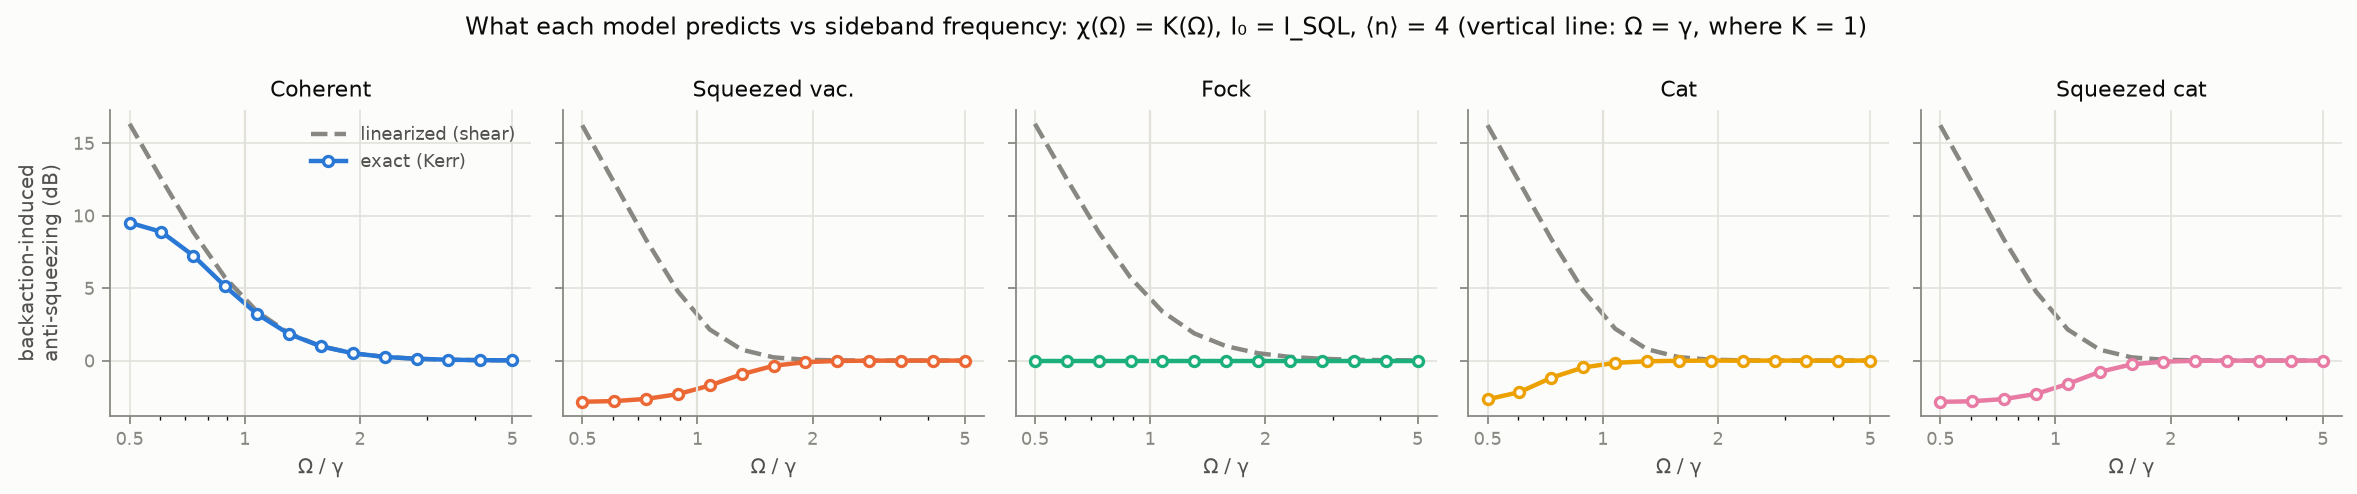
\includegraphics[width=\linewidth]{fig_bridge_freq_prediction.png}
\caption{What each model predicts across the band: backaction-induced
anti-squeezing of the noisiest quadrature (dB above the input state)
versus sideband frequency, with $\chieff(\Omega) = \mathcal{K}(\Omega)$ at
$I_0 = I_{\mathrm{SQL}}$ [Eq.~\eqref{eq:kimble}], for the exact Kerr
(solid, colored) and the linearized shear (dashed, gray). Above
$\Omega \approx 2\gamma$ backaction is negligible and the models agree
trivially; below $\Omega \approx \gamma$ the linearized model predicts a
steeply growing noise ($\mathcal{K} \propto \Omega^{-4}$ in this region)
that the exact model does not produce for any non-Gaussian family (Fock:
exactly none at any frequency). Only the coherent carrier tracks the
linearized prediction into the backaction-dominated band.}
\label{fig:prediction}
\end{figure}

\begin{figure}[t]
\centering
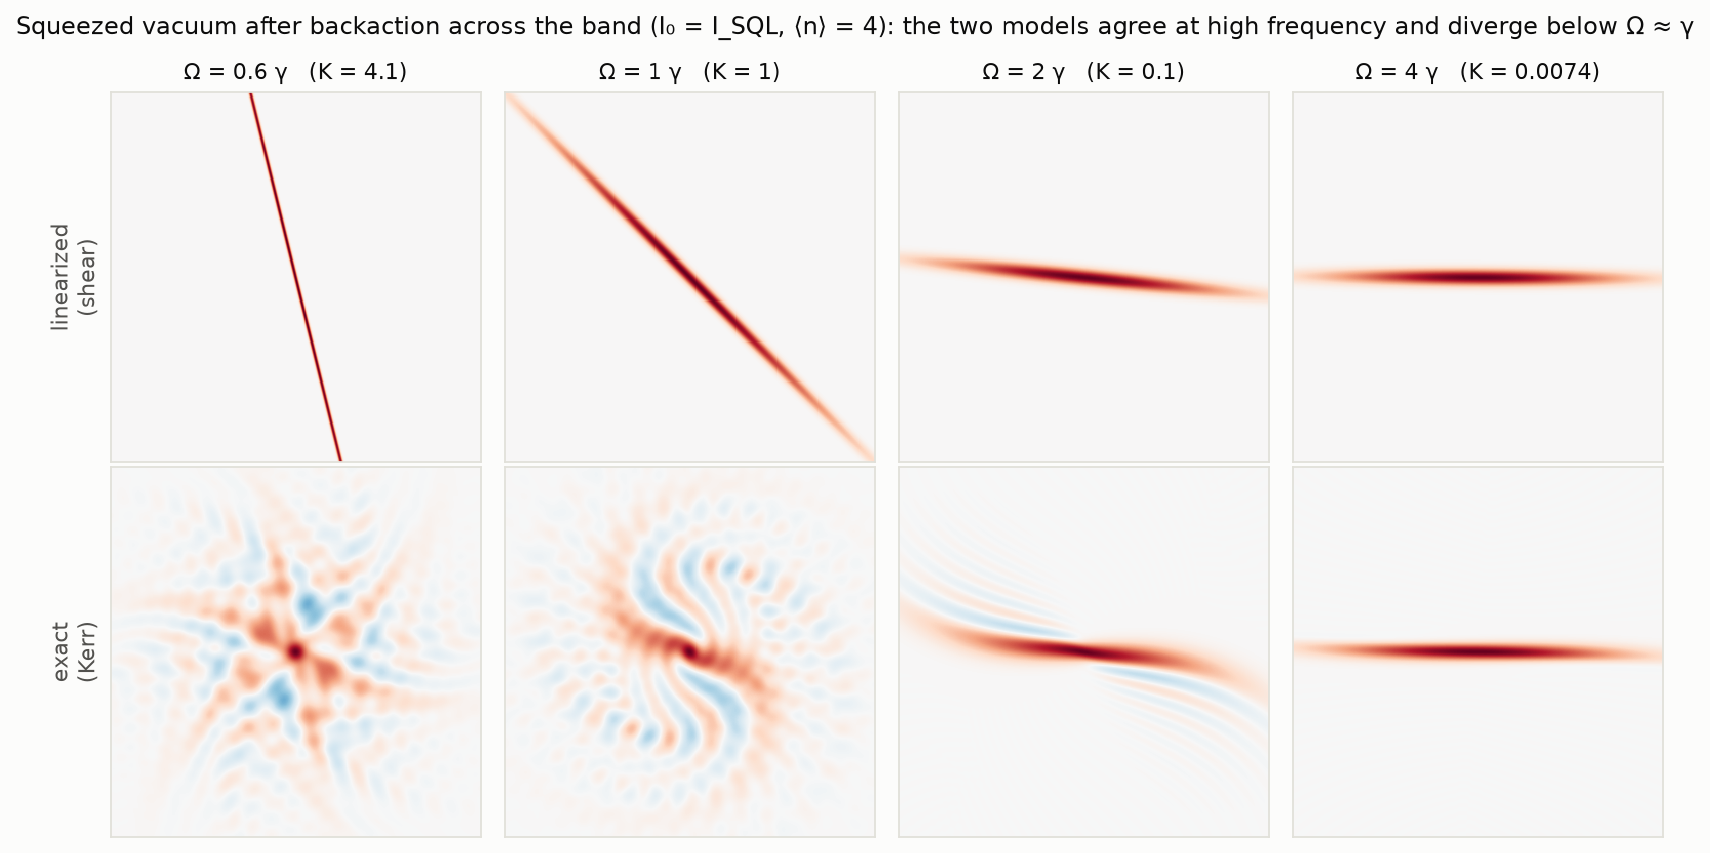
\includegraphics[width=0.9\linewidth]{fig_bridge_freq_wigner.png}
\caption{Squeezed vacuum after backaction at four sideband frequencies
($I_0 = I_{\mathrm{SQL}}$, $\nbar = 4$): linearized shear (top row,
rendered analytically from its covariance --- the linearized output is
Gaussian by definition) versus exact Kerr (bottom row). At
$\Omega = 4\gamma$ ($\mathcal{K} \approx 0.007$) the rows are
indistinguishable; at $2\gamma$ the exact state develops its first
non-Gaussian curl; at and below $\Omega = \gamma$ the exact interaction
wraps the state into interference-rich structures while the linearized
model continues to predict a straight, thinner line.}
\label{fig:wigner}
\end{figure}

\begin{figure}[t]
\centering
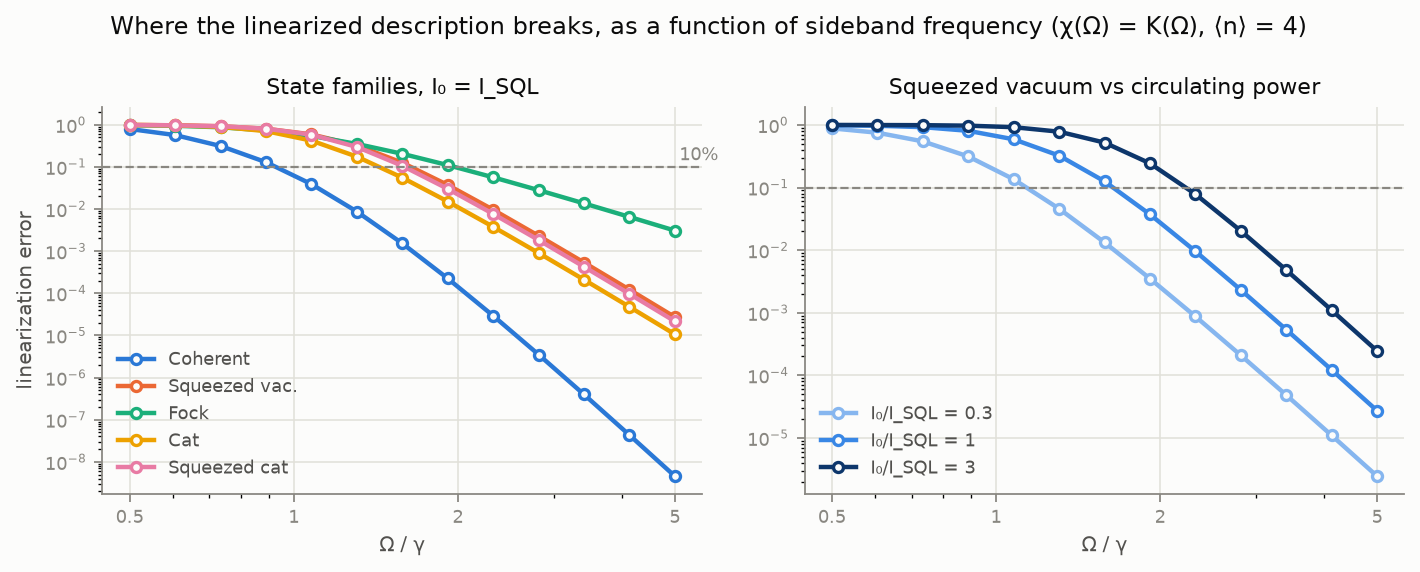
\includegraphics[width=0.95\linewidth]{fig_bridge_freq_error.png}
\caption{Linearization error versus sideband frequency (log--log; dashed
guide at $10\%$). Left: state families at $\nbar = 4$, $I_0 =
I_{\mathrm{SQL}}$. The coherent carrier stays below $10\%$ down to
$\Omega \approx 0.9\gamma$, whereas the non-Gaussian families cross it at
$1.5$--$2\gamma$ (Fock remains above $10^{-2}$ even at $5\gamma$). Right:
the same error for squeezed vacuum at three circulating powers --- raising
the power moves the breakdown frequency up, roughly following the contour
$\mathcal{K}(\Omega) = \mathrm{const}$.}
\label{fig:error}
\end{figure}

Table~\ref{tab:errors} and Figs.~\ref{fig:prediction}--\ref{fig:error}
summarize the comparison. Three mechanisms, one per class of state:

\begin{itemize}
\item \textbf{Coherent: the linearization works and is systematically
improvable.} The error grows quadratically in $\chieff$ and falls as
$1/\nbar$ at fixed $\chieff$ --- the classical-carrier limit becoming
exact. This is the regime the frequency-domain formalism was built for,
and at interferometric photon numbers it is effectively exact.

\item \textbf{Fock: the linearized model hallucinates backaction.} A
number eigenstate has \emph{zero} intensity fluctuations, so there is
nothing to fluctuate the radiation-pressure force:
$U_K|n\rangle$ is a global phase and the exact model produces no
distortion at all. The linearized model, blind to number statistics,
predicts full ponderomotive squeezing; the entire tabulated error is that
phantom prediction, which is why it appears at first order in $\chieff$.

\item \textbf{Cat and squeezed states: no single mean field exists.} The
even cat is a superposition of two carriers $\pm\alpha$; each branch would
linearize well about its own mean field, but the exact interaction bends
the two branches oppositely, and no single linear map represents that.
Squeezed vacuum has $\langle a \rangle = 0$ with
all of its intensity carried by fluctuations, so the ``small parameter''
of the expansion is $\mathcal{O}(1)$ by construction; the resulting
S-shaped curl of the exact output, versus the straight line the linearized
model predicts, is visible across the band in Fig.~\ref{fig:wigner}.
\end{itemize}

\section{Interpretation and caveats}

The linearized description is a mean-field expansion about a c-number
carrier; its small parameter is the ratio of photon-number-fluctuation
scale to carrier amplitude. Coherent states make that ratio $1/\sqrt{\nbar}$;
Fock, cat, and squeezed-vacuum states make it $\mathcal{O}(1)$ --- not
because any carrier decoheres, but because these states have no single
mean field to expand around.

Two caveats bound what this result does and does not show. First, it is a
\emph{single-mode} statement: in a real interferometer the carrier is a
separate, macroscopically populated coherent mode, and the exotic state is
injected into the sideband (dark-port) modes, so the expansion parameter
involves the injected state's moments against the \emph{laser} amplitude,
which is enormous. Our model conflates carrier and sideband; the honest
multi-mode versions of the breakdown are (i) nonlinear force terms
suppressed by the carrier but weighted by the injected state's number
spread, and (ii) the $\hat n^{2}$ interaction coupling sideband
\emph{pairs} at different frequencies --- which is precisely the mechanism
by which per-frequency independence and linearity fail together for
non-Gaussian inputs. Second, as noted above, the covariance-level metric
is charitable, so the quoted breakdown couplings are lower bounds.

\section{What we should do}

\begin{enumerate}
\item \textbf{Keep both interaction forms in the simulation harness.} Use
the shear for frequency-resolved, physically calibrated statements
($\chi = \mathcal{K}(\Omega)$, SQL curves, comparison against the Gaussian
covariance rail) and the Kerr for any conclusion about non-Gaussian states
under backaction. State-comparison results should be reported under both,
with disagreement itself reported as physics.

\item \textbf{Build the two-mode carrier--sideband model next.} An
explicit coherent carrier mode tensored with a quantum sideband mode
carrying the exotic state, coupled through the expanded $\hat n^{2}$
interaction, separates the artifact (``the state had to be its own
carrier'') from the genuine nonlinear corrections, and gives the breakdown
scale as a function of carrier power at fixed injected state.

\item \textbf{Test per-frequency independence directly.} A joint
simulation of $2$--$3$ frequency modes with the pairwise couplings induced
by $\hat n^{2}$, versus the product of single-frequency channels, is the
multi-mode version of this study and the direct answer to where the
independent-frequency description fails for non-Gaussian states. The
single-mode result predicts the relevant coupling scale.

\item \textbf{Tighten the metric.} Repeat the bridge at the level of QFI
for the displacement signal (and, later, state fidelity). Since the
covariance metric is the charitable one, this can only strengthen the
conclusion, and it connects the breakdown directly to sensing performance.

\item \textbf{Port the classical Fisher information (homodyne) tooling to
Python.} Backaction trade-offs of the standard-quantum-limit type live in
fixed-measurement CFI, not in QFI (which is provably blind to the shear
for phase-quadrature signals). This is the prerequisite for honest SQL
statements in either model.

\item \textbf{Calibrate the regime.} Map $\chieff$ to physical
interferometer parameters (circulating power, mass, measurement time) to
locate where a realistic device sits on Fig.~\ref{fig:error} for the
sideband powers at which optimized non-Gaussian states would actually be
injected.
\end{enumerate}

\vspace{1em}
\noindent\textbf{Reproducibility.} All numbers and figures come from the
self-contained \texttt{backaction-study/} folder (branch
\texttt{claude/quantum-sensing-backaction-jn5ty7}):
\texttt{run\_study.py} (experiments E5 and companions;
\texttt{run\_bridge\_frequency()} for the figures shown here),
\texttt{results/bridge\_results.csv},
and the regression test \texttt{test\_kerr\_linearizes\_to\_shear}, which
pins the bridge Eq.~\eqref{eq:bridge} and its $1/\nbar$ convergence.
Abstract-coupling ($\chieff$-axis) versions of all three figures are also
generated (\texttt{results/fig\_bridge*.png}).

\end{document}
